\documentclass{article}
\usepackage[english,russian]{babel}
\usepackage{textcomp}
\usepackage{geometry}
  \geometry{left=2cm}
  \geometry{right=1.5cm}
  \geometry{top=1.5cm}
  \geometry{bottom=2cm}
\usepackage{tikz}
\usepackage{listings}
\usepackage{fancyvrb}
\usepackage{xcolor}
\pagenumbering{gobble}

\lstset{
  language=C++,
  basicstyle=\linespread{1.1}\ttfamily,
  columns=fixed,
  fontadjust=true,
  basewidth=0.5em,
  keywordstyle=\color{blue}\bfseries,
  commentstyle=\color{gray},
  texcl=true,
  stringstyle=\ttfamily\color{orange!50!black},
  showstringspaces=false,
  %numbers=false,
  numbersep=5pt,
  numberstyle=\tiny\color{black},
  numberfirstline=true,
  stepnumber=1,      
  numbersep=10pt,
  backgroundcolor=\color{white},
  showstringspaces=false,
  captionpos=b,
  breaklines=true
  breakatwhitespace=true,
  xleftmargin=.2in,
  extendedchars=\true,
  keepspaces = true,
  tabsize=4,
  upquote=true,
}
\lstset{ literate={~}{{\raisebox{0.5ex}{\texttildelow}}}{1}}

\renewcommand{\thesubsection}{\arabic{subsection}}
\makeatletter
\def\@seccntformat#1{\@ifundefined{#1@cntformat}%
   {\csname the#1\endcsname\quad}%    default
   {\csname #1@cntformat\endcsname}}% enable individual control
\newcommand\section@cntformat{}     % section level 
\newcommand\subsection@cntformat{Задача \thesubsection.\space} % subsection level
\newcommand\subsubsection@cntformat{\thesubsubsection.\space} % subsubsection level
\makeatother

\begin{document}
\title{Семинар \#1: События библиотеки SFML. Домашнее задание.\vspace{-5ex}}\date{}\maketitle
Все задачи нужно решить обязательно с использование только одной сторонней библиотеки -- SFML.


\subsection{Нажатие на клавишу}
Напишите программу, которая рисует на экране круг зелёного цвета. При нажатии клавиши пробел цвет круга должен меняться на красный. Круг должен оставаться красным, пока клавиша пробел зажата. После отпускания клавиши пробел круг должен снова становиться зелёным. Решите эту задачу двумя способами:
\begin{enumerate}
\item Используя статические методы класса \texttt{sf::Keyboard}.
\item Используя события \texttt{sf::Event::KeyPressed} и \texttt{sf::Event::KeyReleased}.
\end{enumerate}

\subsection{Столкновение курсора с прямоугольником}
Напишите программу, которая бы рисовала прямоугольник, цвет которого изменялся бы при наведении на него мышью. Если курсор мыши находится вне прямоугольник, то он должен рисоваться зелёным цветом. Если курсор мыши находится внутри прямоугольника, то красным.
Решите эту задачу двумя способами:
\begin{enumerate}
\item Используя статические методы класса \texttt{sf::Mouse}.
\item Используя событие \texttt{sf::Event::MouseMoved}.
\end{enumerate}
Программа должна работать корректно при изменении размеров окна.
Для обнаружения столкновения фигуры прямоугольника с курсором используйте метод \texttt{getGlobalBounds}, чтобы получить объект типа \texttt{sf::FloatRect}, а затем метод \texttt{contains}.

\subsection{Создание кругов}
Напишите программу, в которой можно создавать круги по нажатию левой кнопки мыши. При нажатии ЛКМ в определённом месте окна должен появляться круг белого цвета, причём центр круга должен совпадать с положением курсора мыши. При нажатии клавиши пробел цвет всех кругов должен изменяться на случайный. Программа должна корректно работать при изменении размеров окна.

Для получения случайного цвета можно использовать следующую функцию:
\begin{lstlisting}
#include <random>
sf::Color getRandomColor()
{
    static std::random_device rd;
    static std::mt19937 gen(rd());
    std::uniform_int_distribution<uint8_t> d(0, 255);
    return sf::Color{d(gen), d(gen), d(gen)};
}
\end{lstlisting}


\subsection{Тумблер}
Создайте класс \texttt{Toggle}, который бы релизовывал элемент интерфейса тумблер (переключатель).
\begin{center}
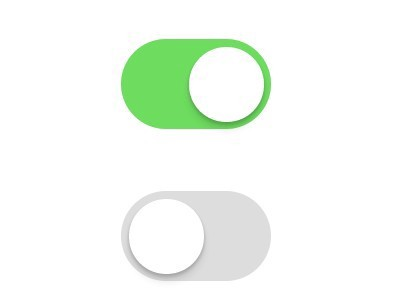
\includegraphics[scale=0.25]{../images/toggle_button.jpeg}
\end{center}
После того, как создадите класс, напишите программу, в которой бы создавалось 10 тумблеров. Все тумблеры должны работать. Программа должна корректно работать при изменении размеров окна.


\subsection{Три слайдера}
Напишите программу, которая создаёт круг и три слайдера. Цвет круга должен меняться при изменении положения ползунков слайдеров. Каждый слайдер должен отвечать за свою компоненту цвета круга (красную, зелёную или синию). Используйте класс \texttt{Slider} из \texttt{classroom\_tasks/code/5gui/2slider}.
\begin{center}
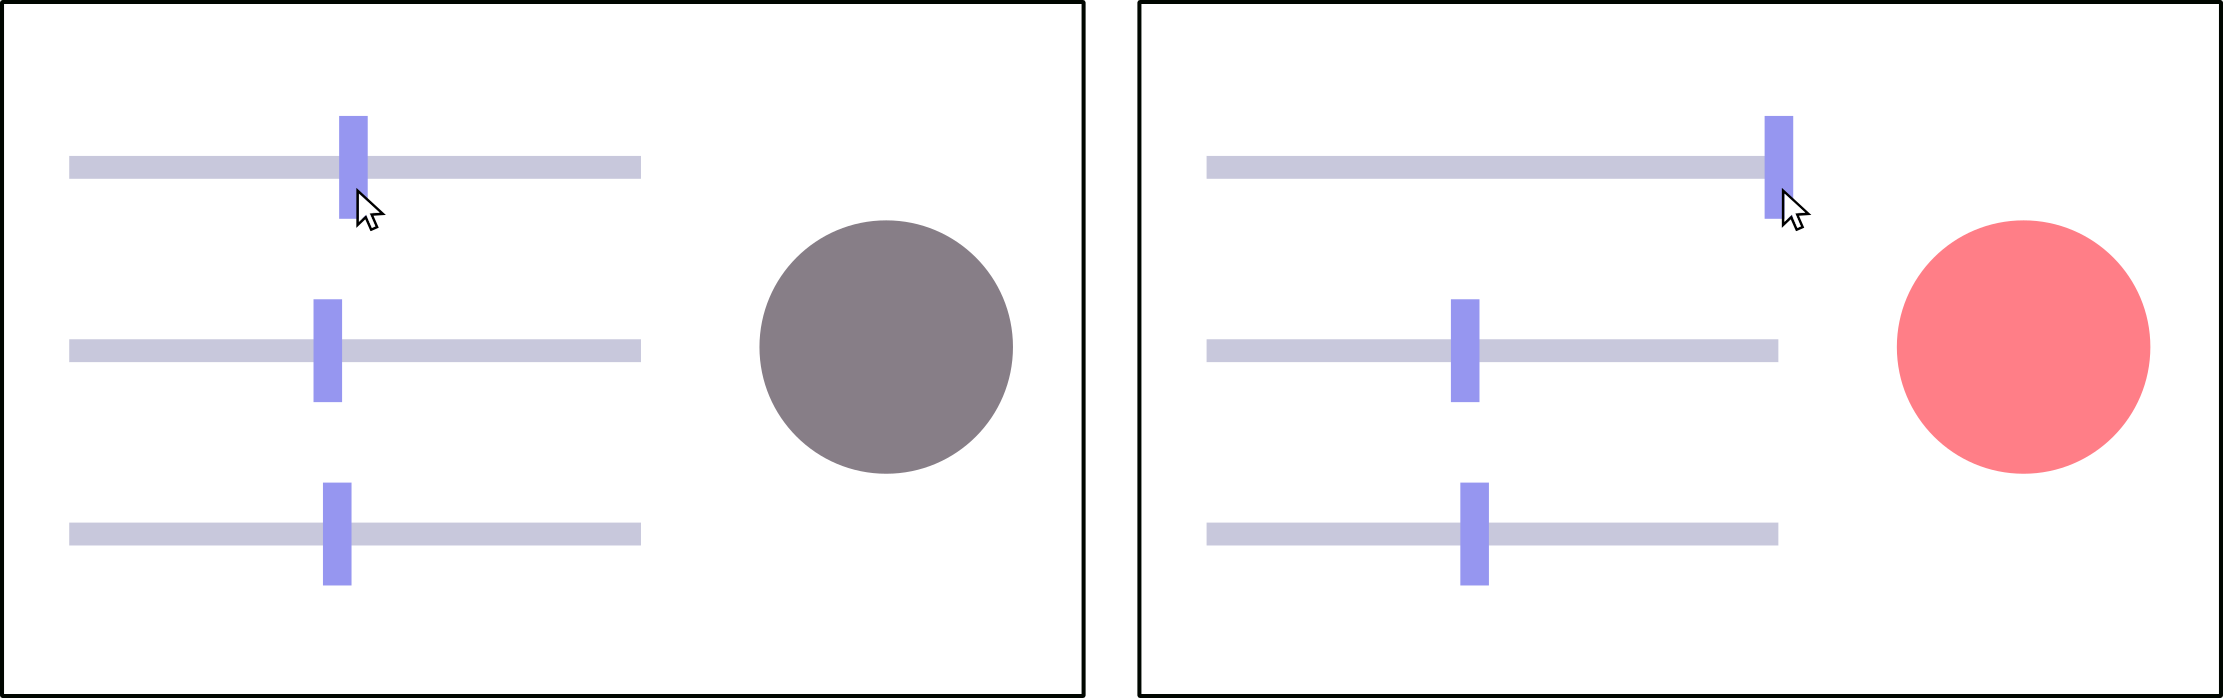
\includegraphics[scale=0.95]{../images/slider_chose_color.png}
\end{center}

\subsection{Выпадающий список}
Создайте класс \texttt{DropList}, который бы релизовывал элемент интерфейса выпадающий список без полосы прокрутки.
\begin{center}
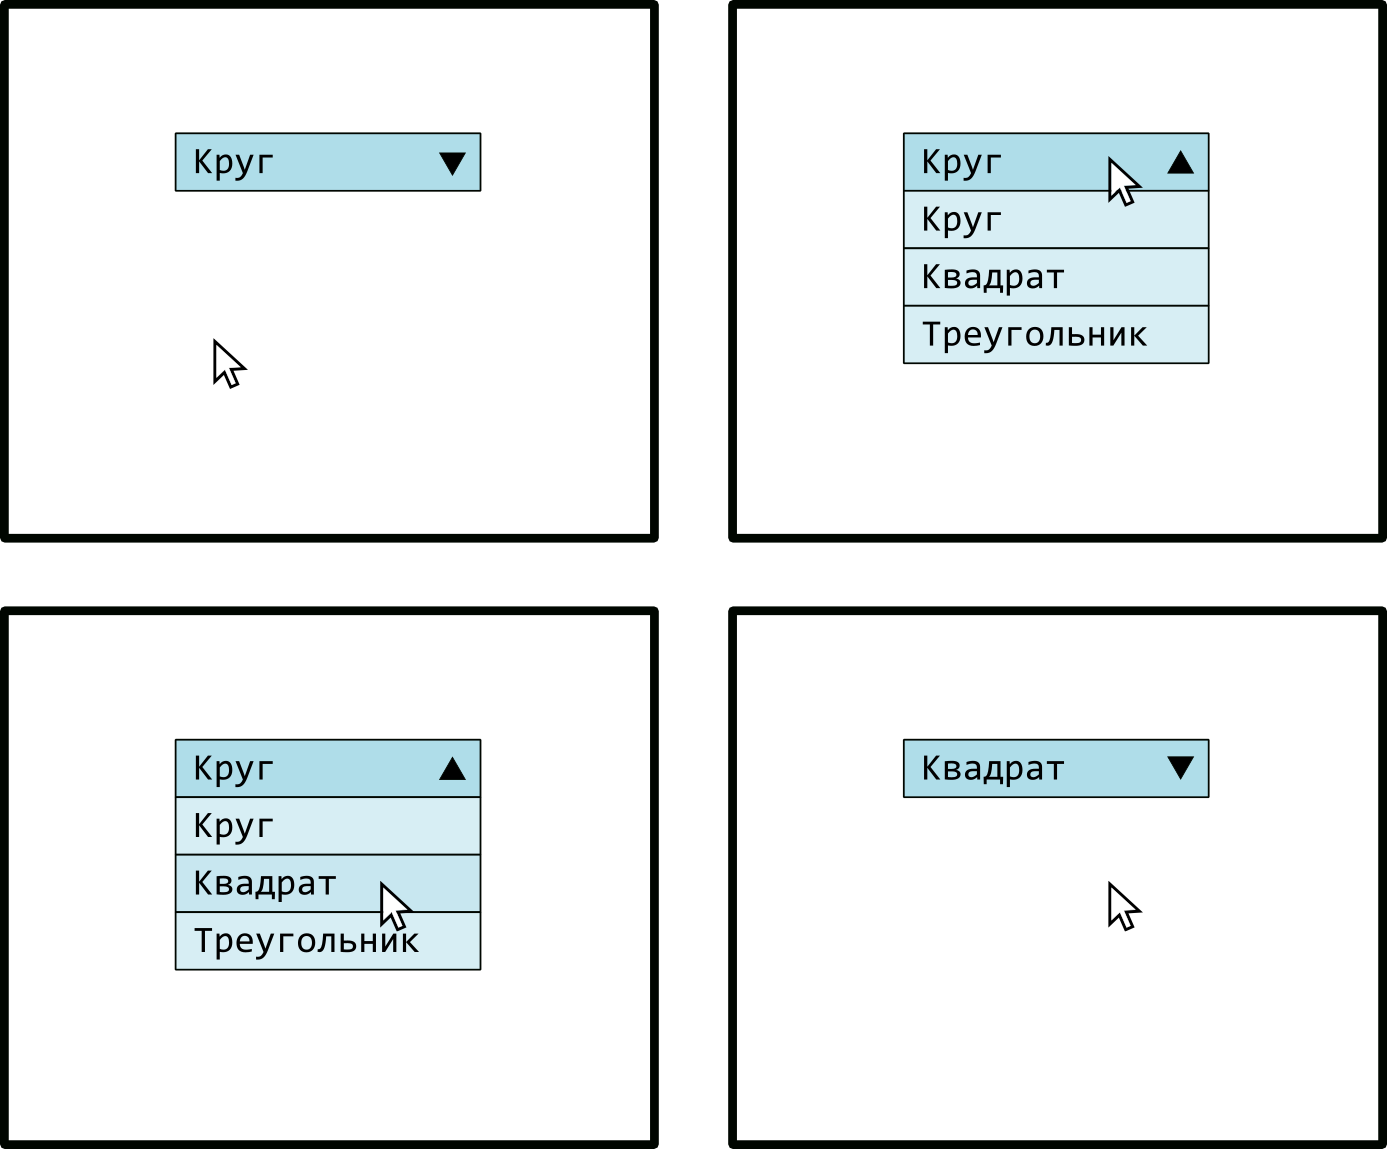
\includegraphics[scale=1]{../images/drop_down_list.png}
\end{center}
После создания класса напишите программу, которая реализует выпадающий список с тремя вариантами: \texttt{Круг}, \texttt{Квадрат} и \texttt{Треугольник}. В зависимости от выбранного в списке варианта, на экране должна отображаться соответствующая фигура: круг, квадрат или треугольник. Нарисовать треугольник можно, используя класс круга: 
\begin{lstlisting}
sf::CircleShape triangle{50, 3};
\end{lstlisting}
Тут мы используем второй параметр конструктора \texttt{sf::CircleShape}, который задаёт количество сторон рисуемого правильного многоугольника. По умолчанию значение этого параметра равно 30, поэтому при рисовании кругов в SFML на самом деле рисуются правильные 30-ти угольники.

\newpage
\section{Необязательные задачи}

\subsection{Столкновение курсора с кругом}
Напишите программу, которая бы рисовала круг, цвет которого изменялся бы при наведении на него мышью. Если курсор мыши находится вне круга, то круг должен рисоваться зелёным цветом. Если курсор мыши находится внутри круга, то круг должен рисоваться красным цветом.

\subsection{Select Move Delete}
 В папке \texttt{select\_move\_delete/} содержится заготовка исходного кода для этого задания. В этой программе есть несколько объектов(кругов), которые можно выделять. Выделение происходит по нажатию левой клавиши мыши. Зажав клавишу \texttt{Ctrl} можно выделить несколько объектов. Также в программе реализован прямоугольник выделения (но он пока не выбирает объекты). Левой кнопкой мыши с зажатой клавишей левый \texttt{Alt} можно создать круг случайного размера. Добавьте следующие возможности в программу:
\begin{itemize}
\item Задание случайного цвета. При нажатии клавиши пробел цвет всех выделенных шаров должен меняться на случайный. Для этого понадобится добавить поле \texttt{color} в класс \texttt{Ball}.

\item Выделение объектов с помощью прямоугольника выделения. Прямоугольник выделения должен рисоваться только если нажатие мыши произошло вне кругов. Все объекты, полностью находящиеся внутри прямоугольника выделения, на момент отпускания левой кнопки мыши должны выделяться. Объекты должны выделяться во время изменения прямоугольника, а не только при отпускании кнопки мыши.

\item Перемещение всех выделенных объектов при зажатии левой клавиши мыши и её движении. Перемещаться должны все выделенные объекты параллельно (также как перемещаются несколько выделенных значков на рабочем столе). Прямоугольник выделения при этом рисоваться не должен.

\item При нажатии клавиши \texttt{Delete}, все выделенные объекты должны удаляться. Чтобы удалить элемент из \texttt{std::list} используйте итераторы и метод \texttt{erase}. При удалении элемента \texttt{std::list} нужно внимательно следить за тем, чтобы не испортить итераторы.

\item В папке \texttt{code/5gui/5context\_menu} содержится реализация контекстного меню -- класс \texttt{ContextMenu}. Используйте этот класс чтобы добавить контекстное меню в программу. Оно должно открываться при нажатии правой кнопки мыши. Добавьте следующие варианты в меню:
\begin{itemize}
\item \texttt{Delete} - при нажатии на выделенные объект правой кнопкой мыши и выборе этого варианта все выделенные объекты должны удаляться.
\item \texttt{Create} - при нажатии на любое место и выборе этого варианта должнен создаваться новый случайный круг.
\item \texttt{Random Color} -- все выделенные объекты должны окрашиваться в случайный цвет.
\item \texttt{Increase} -- все выделенные объекты должны увеличиваться на 25 процентов.
\item \texttt{Decrease} -- все выделенные объекты должны уменьшаться на 25 процентов.
\end{itemize}

\item \textbf{Copy Paste Cut} Добавьте возможность копирования, вставки и вырезания объектов. Вызов этих операций должен происходить в контекстном меню или с помощью комбинаций клавиш \texttt{Ctrl-C}, \texttt{Ctrl-V} и \texttt{Ctrl-X}.
\end{itemize}


\end{document}